\documentclass[11pt,a4paper]{article}
\usepackage[main=italian,provide=*]{babel}
\usepackage[utf8]{inputenc}
\usepackage[T1]{fontenc}
\usepackage{amsmath,amssymb}
\usepackage{geometry}
\geometry{margin=2.7cm}
\usepackage{booktabs}
\usepackage{array}
\usepackage{caption}
\usepackage{tikz}
\usepackage{pgfplots}
\pgfplotsset{compat=1.18}
\usepackage[colorlinks=true,linkcolor=blue,citecolor=blue]{hyperref}

\title{Dimero di spin per la simulazione VQE:\\
inquadramento, termine di Dzyaloshinskii--Moriya\\
e piano operativo per il dimero $N=2$\\[6pt]
\large Sintesi ragionata della fase preliminare}
\author{Samuele \\ Relatore: Prof. Alessandro Chiesa}
\date{24 giugno 2026 \\ \small Riferimento concettuale: M.\ Crippa et al., \emph{Magnetochemistry} \textbf{7}, 117 (2021); materiale del corso 6 -- Applications.}

\begin{document}
\maketitle

\begin{abstract}
\noindent Questo documento raccoglie e organizza in forma coerente quattro punti emersi
nella fase preliminare del lavoro di tesi. Nell'ordine: (i) l'inquadramento del problema
-- argomento, Hamiltoniana del dimero da cui si parte, struttura in due parti; (ii)
l'effetto del termine di Dzyaloshinskii--Moriya sulla repulsione tra i livelli e
sull'incrocio del fondamentale in $B/J=2$; (iii) l'analisi della degenerazione residua
del tripletto a campo nullo e della sua irrilevanza per il fondamentale; (iv)
l'aggiornamento di scope (sessione di settembre, entrambe le topologie per $N=3$) e il
piano operativo per il dimero $N=2$. I contenuti sono quelli discussi nei rispettivi
passaggi; le figure illustrano i risultati gi\`a stabiliti.
\end{abstract}

\tableofcontents

\section{Inquadramento del problema}

\subsection{Argomento}

Il lavoro riguarda la simulazione quantistica di sistemi molecolari su hardware
quantistico, declinata su sistemi di spin-1/2 di tipo Heisenberg (nanomagneti
molecolari). Ogni spin-1/2 si mappa direttamente su un qubit: l'Hamiltoniana \`e gi\`a
una somma di prodotti di Pauli, quindi non serve alcun mapping fermionico. Il metodo
\`e il VQE: si costruisce uno stato di prova parametrizzato
$|\psi(\vec\theta)\rangle=U(\vec\theta)|0\rangle$ e se ne minimizza il valore di
aspettazione
$$\langle H\rangle_{\vec\theta} = \langle\psi(\vec\theta)|H|\psi(\vec\theta)\rangle$$
con un ciclo quantistico-classico, confrontando il risultato con la diagonalizzazione
esatta. Riferimento concettuale: Crippa et al.\ (2021). Le reti neurali (NQS) sono
fuori scope.

\subsection{Hamiltoniana del dimero}

Il punto di partenza \`e l'esempio ``VQE on a spin dimer'' del materiale del corso:
\begin{equation}
H = J_x X_1X_2 + J_y Y_1Y_2 + J_z Z_1Z_2 + b(Z_1+Z_2), \qquad s_i=\frac12(X_i,Y_i,Z_i),
\end{equation}
nel caso isotropo $J_x=J_y=J_z\equiv J$, con parametro di controllo $b/J$. Posto
$\vec S=\vec s_1+\vec s_2$ si separa $H=H_1+H_2$ con
\begin{equation}
H_1 = J(X_1X_2+Y_1Y_2+Z_1Z_2) = 2J\big(\vec S^2-\vec s_1^2-\vec s_2^2\big) = 2J\,S(S+1)-3J,
\end{equation}
\begin{equation}
H_2 = b(Z_1+Z_2) = 2b\,S_z, \qquad [H_1,H_2]=0,
\end{equation}
da cui lo spettro analitico, riferimento esatto per validare il VQE,
\begin{equation}
E(S,M) = 2J\,S(S+1) - 3J + 2bM.
\end{equation}
Esplicitamente: il singoletto $S=0$, $M=0$ ha $E=-3J$; il tripletto $S=1$ ha
$E=J+2bM$ con $M\in\{-1,0,+1\}$, cio\`e $\{J-2b,\,J,\,J+2b\}$. Il fondamentale passa dal
singoletto allo stato $|\!\downarrow\downarrow\rangle=|11\rangle$ in $b/J=2$; a campo
alto il fondamentale \`e quello banalmente polarizzato. La convenzione adottata \`e
quella del materiale del corso ($J$ davanti a $X_1X_2+Y_1Y_2+Z_1Z_2$); Crippa et al.\
usano $2J\sum_{\langle i,j\rangle}\vec s_i\cdot\vec s_j+B\sum_i s_i^z$: stesso modello a
meno di fattori 2.

\subsection{Struttura in due parti}

\paragraph{Parte 1 -- sistema chiuso (senza rumore).} Stato puro $|\psi\rangle$,
evoluzione unitaria. Si parte dal dimero $N=2$ e si estende a $N=3$. VQE su
simulatore statevector, confronto con la soluzione esatta, calcolo di osservabili
(p.es.\ la magnetizzazione $M_z=(Z_1+Z_2)/2$) e della fidelity
$\mathcal F=|\langle\psi_0|\psi(\tilde{\vec\theta})\rangle|$.

\paragraph{Parte 2 -- sistema aperto (con rumore).} Formalismo dell'operatore densit\`a
$\rho$ (stati misti, dinamica non unitaria), con modelli di rumore approssimati in
Qiskit: $T_1$, $T_2$, errori di gate e di lettura.

\begin{center}
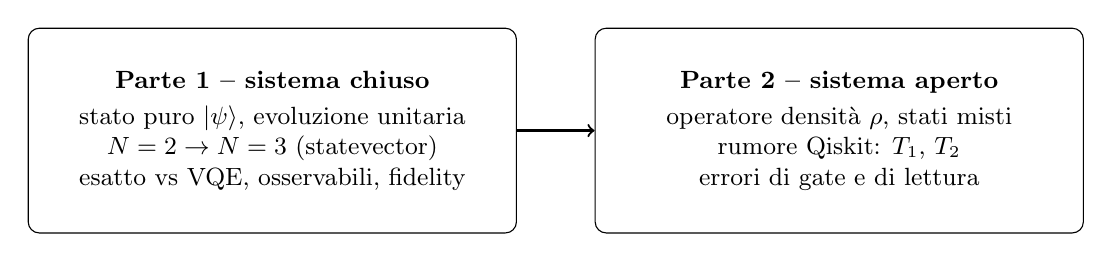
\begin{tikzpicture}[every node/.style={font=\small,align=center}, box/.style={draw,rounded corners,minimum width=6.2cm,minimum height=2.6cm}]
 \node[box] (p1) at (0,0) {\textbf{Parte 1 -- sistema chiuso}\\[2pt]
   stato puro $|\psi\rangle$, evoluzione unitaria\\
   $N=2\to N=3$ (statevector)\\
   esatto vs VQE, osservabili, fidelity};
 \node[box] (p2) at (7.2,0) {\textbf{Parte 2 -- sistema aperto}\\[2pt]
   operatore densit\`a $\rho$, stati misti\\
   rumore Qiskit: $T_1$, $T_2$\\
   errori di gate e di lettura};
 \draw[->,thick] (p1) -- (p2);
\end{tikzpicture}
\captionof{figure}{Struttura in due parti del lavoro: il sistema chiuso (statevector)
\`e il nucleo quantitativo; il sistema aperto ($\rho$) ne \`e l'estensione con rumore.}
\end{center}

\section{Il termine di Dzyaloshinskii--Moriya e la repulsione tra livelli}

Il notebook di partenza contiene, oltre alla (1) isotropa, un termine extra
\begin{equation}
H_D = D\,(X_1Z_2 - Z_1X_2) = -4D\,(\vec s_1\times\vec s_2)_y, \qquad D=0.2,
\end{equation}
cio\`e un'interazione antisimmetrica di Dzyaloshinskii--Moriya con vettore DM lungo
$\hat y$. La domanda \`e se questo termine aumenti o diminuisca la repulsione tra i
livelli, e se serva a evitarne l'incrocio. La risposta \`e affermativa, ma con una
precisazione sul meccanismo: il termine crea una repulsione dove la simmetria la
vietava, non rende pi\`u repulsivi livelli che gi\`a si respingevano.

\subsection{Cosa mostra il calcolo}

In $B/J=2$ il singoletto ($S=0$, $M=0$, $E=-3J$) e il tripletto $M=-1$
($E=J-2b$) hanno la stessa energia. Con $D=0$ il gap tra fondamentale e primo
eccitato si chiude esattamente a zero in quel punto; con $D=0.2$ resta finito
(minimo $\Delta\simeq0.57$). \`E un incrocio che diventa evitato (Figure 2 e 3).

\begin{center}
\begin{tabular}{@{}ccc@{}}
\toprule
$B/J$ & gap con $D=0$ & gap con $D=0.2$ \\
\midrule
1.90 & 0.200 & 0.603 \\
2.00 & 0.000 & 0.565 \\
2.10 & 0.200 & 0.597 \\
\bottomrule
\end{tabular}
\captionof{table}{Gap fondamentale--primo eccitato vicino a $B/J=2$: nullo per $D=0$
(incrocio vero), finito per $D=0.2$ (anticrossing).}
\end{center}

\begin{center}
\begin{tikzpicture}
\begin{axis}[width=13cm,height=6.5cm,xlabel={$B/J$},ylabel={$E/J$},
  xmin=0,xmax=5,ymin=-9,ymax=6, legend pos=north west, legend style={font=\footnotesize}]
\addplot[gray,dashed,thick] table[x=B,y=E0] {fig_spettro.dat};
\addplot[gray,dashed,thick] table[x=B,y=E1] {fig_spettro.dat};
\addplot[gray,dashed,thick] table[x=B,y=E2] {fig_spettro.dat};
\addplot[gray,dashed,thick] table[x=B,y=E3] {fig_spettro.dat};
\addplot[black,thick] table[x=B,y=E0] {fig_spettro.dat};
\addplot[red,dashed,thick] table[x=B,y=E0d] {fig_spettro.dat};
\draw[dotted] (axis cs:2,-9) -- (axis cs:2,6);
\legend{livelli ($D=0$),,,, GS ($D=0$), GS ($D=0.2$)}
\end{axis}
\end{tikzpicture}
\captionof{figure}{Spettro $E/J$ in funzione di $B/J$. Con $D=0$ il fondamentale
(nero) ha un incrocio in $B/J=2$ (cambio di pendenza, dal singoletto piatto allo stato
$M=-1$ discendente); con $D=0.2$ il fondamentale (rosso tratteggiato) passa con
continuit\`a: l'incrocio \`e diventato evitato.}
\end{center}

\subsection{Perch\'e: una questione di simmetria}

L'Hamiltoniana isotropa $H_0$ commuta con $S_z=(Z_1+Z_2)/2$. I due stati che si
incrociano hanno numeri quantici diversi ($M=0$ il singoletto, $M=-1$ il tripletto),
quindi non hanno elemento di matrice:
$$\langle S{=}0,M{=}0|H_0|S{=}1,M{=}{-}1\rangle = 0 \qquad \text{(diverso $M$)}.$$
Senza accoppiamento i livelli si attraversano liberamente: l'incrocio \`e protetto
dalla simmetria assiale, gap nullo. Il termine DM rompe proprio quella simmetria; a
$D=0.2$, il calcolo d\`a
$$\|[H_D,S_z]\| = 0.57, \qquad \|[H_D,S^2]\| = 1.13 \qquad \text{(norma di Frobenius)},$$
quindi $H_D$ non conserva $M$ e pu\`o connettere stati con $M$ diverso. Compare un
elemento di matrice fuori diagonale tra singoletto e tripletto $M=-1$, i due stati si
ibridano e l'incrocio diventa evitato con gap $\Delta\sim2|\langle0|H_D|\!\downarrow\downarrow\rangle|$.

\begin{center}
\begin{tikzpicture}
\begin{axis}[width=13cm,height=5.5cm,xlabel={$B/J$},ylabel={gap $\Delta/J$},
  xmin=0,xmax=5,ymin=0,ymax=3.2, legend pos=north east, legend style={font=\footnotesize}]
\addplot[black,thick] table[x=B,y=gap0] {fig_gap.dat};
\addplot[red,dashed,thick] table[x=B,y=gapd] {fig_gap.dat};
\legend{$D=0$, $D=0.2$}
\end{axis}
\end{tikzpicture}
\captionof{figure}{Gap fondamentale--primo eccitato. Con $D=0$ si annulla in $B/J=2$
(degenerazione del fondamentale); con $D=0.2$ resta finito (minimo $\simeq0.57$):
\`e la repulsione che il termine DM introduce.}
\end{center}

\subsection{Risposta diretta}

La repulsione aumenta nel senso preciso che il gap nel punto di incrocio passa da 0 a
un valore finito: prima del termine non c'era repulsione l\`i (incrocio vero), $H_D$ la
introduce. Lo scopo \`e rimuovere la degenerazione del fondamentale in $B/J=2$, cos\`i
che il ground state resti unico e a gap finito su tutto il range: \`e la condizione
per un test VQE pulito (fidelity ben definita, fondamentale che varia con continuit\`a,
nessuna ambiguit\`a nell'autostato al punto di degenerazione). Una precisazione
terminologica: il termine non rende pi\`u repulsivi livelli che gi\`a si respingevano,
ma agisce solo dove c'erano incroci protetti, trasformandoli in anticrossing.

\subsection{Una firma osservabile: la magnetizzazione}

L'anticrossing ha un riflesso diretto sulla magnetizzazione del fondamentale
$\langle M_z\rangle$. Con $D=0$ essa vale esattamente $0$ (singoletto) sotto $B/J=2$
e $-1$ (tripletto $M=-1$) sopra, con un salto netto all'incrocio -- la firma della
transizione del primo ordine. Con $D=0.2$ varia con continuit\`a attraverso $B/J=2$:
il gradino diventa un crossover liscio (Figura 4).

\begin{center}
\begin{tikzpicture}
\begin{axis}[width=13cm,height=5.5cm,xlabel={$B/J$},ylabel={$\langle M_z\rangle$},
  xmin=0,xmax=5,ymin=-1.05,ymax=0.05, legend pos=south east, legend style={font=\footnotesize}]
\addplot[black,thick] table[x=B,y=Mz0] {fig_mag.dat};
\addplot[red,dashed,thick] table[x=B,y=Mzd] {fig_mag.dat};
\legend{$D=0$ (salto), $D=0.2$ (crossover)}
\end{axis}
\end{tikzpicture}
\captionof{figure}{Magnetizzazione del fondamentale $\langle M_z\rangle$. Il gradino
netto in $B/J=2$ ($D=0$) diventa un crossover continuo con il termine DM ($D=0.2$).}
\end{center}

\section{L'altra degenerazione: il tripletto a campo nullo}

Resta da verificare l'altro punto degenere dello spettro, quello del tripletto a
$B=0$, e se il termine $D$ lo tocchi. Si comporta in modo diverso dall'incrocio in
$B/J=2$.

\subsection{Cosa dicono i numeri}

A $B=0$ con $D=0$ il tripletto \`e tre volte degenere a $E=J=1$; con $D=0.2$ la
degenerazione si rompe solo parzialmente:
$$D=0:\ [-3.000,\,1.000,\,1.000,\,1.000], \qquad D=0.2:\ [-3.040,\,1.000,\,1.000,\,1.040].$$
Restano due livelli a $1.000$ e uno sale a $1.040$. Lo split \`e $O(D^2)\sim0.04$,
molto pi\`u piccolo del gap $\simeq0.57$ aperto nel caso $B/J=2$. La degenerazione a
$B=0$ \`e di natura diversa: non l'incrocio di due multipletti distinti, ma i tre
stati dello stesso tripletto $S=1$, degeneri a campo nullo.

\subsection{Perch\'e solo parzialmente: $H_D$ \`e cieco al tripletto}

Il termine $H_D\propto(\vec s_1\times\vec s_2)_y$ \`e antisimmetrico per scambio dei
due spin, mentre gli stati di tripletto sono simmetrici. Detto $P_{12}$ l'operatore di
scambio ($P_{12}=+1$ sul tripletto, $-1$ sul singoletto) e poich\'e
$P_{12}H_DP_{12}^{-1}=-H_D$:
\begin{equation}
\langle t|H_D|t'\rangle = \langle t|P_{12}^{-1}(P_{12}H_DP_{12}^{-1})P_{12}|t'\rangle = (+1)(-1)(+1)\langle t|H_D|t'\rangle = -\langle t|H_D|t'\rangle = 0.
\end{equation}
Il blocco $3\times3$ di $H_D$ nel sottospazio di tripletto \`e dunque identicamente
nullo: nessuno split al primo ordine. L'unico canale \`e il secondo ordine, via
accoppiamento col singoletto (parit\`a di scambio opposta). Ma $H_D$ cambia $M$ di
$\pm1$, e il singoletto ha $M=0$:
$$\langle00\,(M{=}{+}1)|H_D|s\rangle = -1.41\,D, \quad \langle11\,(M{=}{-}1)|H_D|s\rangle = -1.41\,D, \quad \langle M{=}0\,\text{trip}|H_D|s\rangle = 0.$$
Solo gli stati $M=\pm1$ vedono il singoletto. A $B=0$: il tripletto $M=0$ resta
esattamente a $E=J=1$ (disaccoppiato, $\Delta M$ proibito); la combinazione
antisimmetrica $(|00\rangle-|11\rangle)/\sqrt2$ resta anch'essa a $1$ (ortogonale
all'accoppiamento); solo la simmetrica $(|00\rangle+|11\rangle)/\sqrt2$ \`e spinta in
su (a $1.040$) e il singoletto in gi\`u (a $-3.040$). Resta una degenerazione residua
2-volte (Figura 5).

\begin{center}
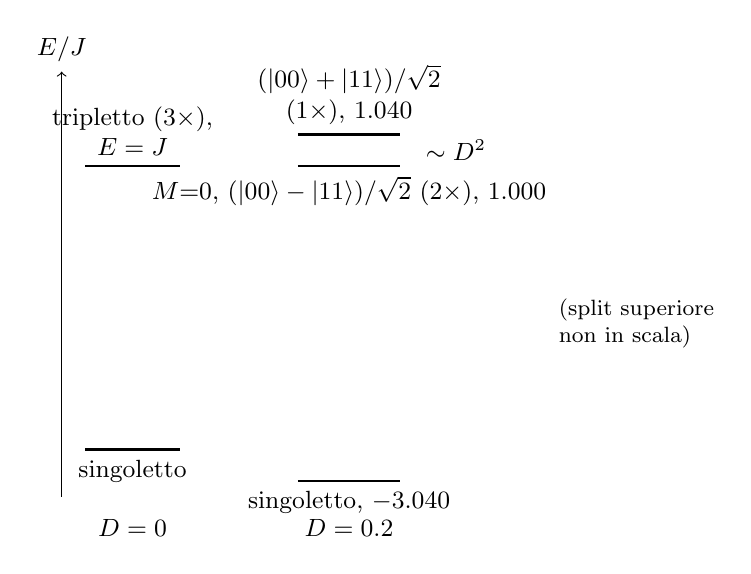
\begin{tikzpicture}[scale=1.0, every node/.style={font=\small}]
 \draw[->] (0,-1.2) -- (0,4.2) node[above]{$E/J$};
 \draw[thick] (0.3,3.0) -- (1.5,3.0) node[midway,above,align=center]{tripletto ($3\times$),\\ $E=J$};
 \draw[thick] (0.3,-0.6) -- (1.5,-0.6) node[midway,below]{singoletto};
 \node at (0.9,-1.6) {$D=0$};
 \draw[thick] (3.0,3.4) -- (4.3,3.4) node[midway,above,align=center]{$(|00\rangle+|11\rangle)/\sqrt2$\\ ($1\times$), $1.040$};
 \draw[thick] (3.0,3.0) -- (4.3,3.0) node[midway,below,align=center]{$M{=}0$, $(|00\rangle-|11\rangle)/\sqrt2$ ($2\times$), $1.000$};
 \draw[thick] (3.0,-1.0) -- (4.3,-1.0) node[midway,below]{singoletto, $-3.040$};
 \node at (3.65,-1.6) {$D=0.2$};
 \node[right] at (4.5,3.2) {$\sim D^2$};
 \node[align=left, font=\footnotesize] at (7.3,1.0) {(split superiore\\ non in scala)};
\end{tikzpicture}
\captionof{figure}{Livelli a $B=0$. La degenerazione 3-volte del tripletto ($D=0$) si
rompe solo parzialmente con $D=0.2$: due stati restano a $E=J$, uno sale di
$O(D^2)$; il singoletto (fondamentale) scende leggermente e resta isolato.}
\end{center}

\subsection{Conseguenza per il VQE}

La degenerazione residua a $B=0$ \`e negli stati eccitati, non nel fondamentale: il
GS \`e il singoletto, non degenere e ben separato ($-3.04$ contro $1.00$). A
differenza dell'incrocio in $B/J=2$, che era sul fondamentale, non disturba il
targeting del ground state. Il termine $D$ pulisce l'unica degenerazione
problematica (quella del fondamentale in $B/J=2$) e lascia intatta quella eccitata
di $B=0$, innocua per il confronto VQE--esatto sull'energia fondamentale.

\section{Aggiornamento di scope e piano operativo}

Due nodi di scope sono chiusi: sessione di settembre come traguardo, e $N=3$ con
entrambe le topologie (catena aperta e anello/triangolo) confermate dal relatore.

\subsection{Implicazioni della sessione di settembre}

Con circa tre mesi a disposizione, di cui le ultime settimane assorbite dalla
stesura, lo scope si calibra cos\`i:
\begin{itemize}
\item \textbf{Parte 1 (chiuso)} \`e il nucleo quantitativo: dimero $N=2\to N=3$ in
entrambe le topologie, dove devono stare i risultati solidi (esatto vs VQE, fidelity,
osservabili).
\item \textbf{Parte 2 (rumore)} resta dimostrativa, non esaustiva: $T_1/T_2$, errori
di gate e di lettura sul solo dimero (al pi\`u $N=3$ catena), per mostrare il degrado
e il formalismo di $\rho$, senza inseguire mitigazione del rumore o hardware reale.
\end{itemize}
Le due topologie per $N=3$ raddoppiano il lavoro di Parte 1 (in particolare il
triangolo frustrato), quindi tenere leggera la Parte 2 \`e la scelta coerente col
vincolo temporale.

\subsection{Piano operativo per il dimero $N=2$}

\begin{enumerate}
\item Hamiltoniana parametrica $H(b,D)$ come singolo \texttt{SparsePauliOp}: sorgente
unica che alimenta sia la diagonalizzazione esatta sia il VQE, evitando incoerenze.
\item Benchmark esatto sull'intero range: spettro, fondamentale, magnetizzazione
$\langle M_z\rangle$, con verifica contro gli autovalori analitici (4) (caso $D=0$).
\item Scheletro VQE pulito in Qiskit 2.x: ansatz + \texttt{StatevectorEstimator} +
\texttt{scipy.optimize.minimize}, senza API deprecate (\texttt{qiskit\_algorithms},
\texttt{AerEstimator}).
\item Confronto: energia VQE vs esatta, fidelity, osservabili sul fondamentale
variazionale.
\end{enumerate}
Il termine $D$ \`e tenuto come parametro: default $D=0$ (l'esatto coincide con gli
autovalori analitici e valida la baseline), $D=0.2$ come variante per esibire
l'anticrossing.

\subsection{Stato del benchmark esatto}

Il modulo di benchmark \`e impostato attorno a una sorgente unica e validato in modo
indipendente: gli autovalori numerici coincidono con quelli analitici a precisione
macchina ($\max|E_{\rm num}-E_{\rm analitico}|=0$ su tutto il range, $D=0$), e la
magnetizzazione riproduce il salto ($D=0$) e il crossover ($D=0.2$) delle Figure~4.
Il nucleo del modulo \`e:

{\small
\begin{verbatim}
from qiskit.quantum_info import SparsePauliOp

def dimer_hamiltonian(b, J=1.0, D=0.0):
    # sorgente unica: stesso operatore per benchmark esatto e VQE
    labels = ["XX", "YY", "ZZ", "ZI", "IZ", "XZ", "ZX"]
    coeffs = [J, J, J, b, b, D, -D]
    return SparsePauliOp(labels, coeffs)
\end{verbatim}
}

La diagonalizzazione esatta usa \texttt{numpy.linalg.eigh} (matrice hermitiana:
autovalori reali e gi\`a ordinati, il primo \`e il fondamentale), e un self-test
verifica automaticamente lo spettro numerico contro l'analitico con tolleranza
$<10^{-10}$.

\subsection{Prossimo passo}

Lo scheletro VQE pulito (passo 3): rifattorizzazione dal pattern deprecato
(\texttt{qiskit\_algorithms.VQE + AerEstimator}) al pattern moderno
\texttt{StatevectorEstimator + scipy.optimize.minimize}, con l'ansatz
hardware-efficient costruito esplicitamente.

\end{document}
